\cotefile{158}
\scanpage{53}
\mspage{7}
% @ top, line 1 | text
Comme corollaire, on a ceci

% @ upper half, lines 2–8 | text
\uline{Proposition 2} Soit $X$ une catégorie \uline{finie} pseudo-cofiltrante, \deleted{\unsure{Donc que|Donc qui}} et soit $X_0$ la \inserted{\unsure{ss-|ss|est}}catégorie ouverte de $X$ formée des \inserted{plus petits} objets de $X$ (NB les hyp. impliquent $X_0\ne\varnothing$), car $X_0$ est $0$-connexe). Supposons que $X_0$ soit $1$-connexe.

% @ middle, lines 9–13 | text
Alors $X$ est cofiltrante (donc tout objet $0$-connexe de $X$ est $\infty$-connexe, et plus \unsure{génér.lt|générlt} asphérique pour tt \deleted{\unsure{dériseur|dériveur}} localiseur fondamental $W$ satisfaisant $W(\unsure{8|\delta})$).

% @ lower third, lines 14–20 and foot | text
\inserted{A fortiori :} \uline{Corollaire} Soit $X$ une catégorie \uline{finie} telle que tout objet $0$-connexe de $X^\wedge$ soit $1$-connexe (p. ex. telle que $X^\circ$ soit tot. $W$-asphérique, où $W$ est un loc. fondamental tel que $W\subset\mathbb{W}_1$). Alors $X$ est cofiltrante, i.e. $X^\circ$ est filtrante (et tt objet de $X^\wedge$ est $\infty$-connexe).
% archive sheet number: 52
\scanpage{54}
\mspage{8}
% @ top, lines 1–3 | text
\handwritten{En effet, on \unsure{a|se} vu que l'hyp. implique que $X$ est pseudo-cofiltrante, et on applique la proposition 2.}

% printed form
% Letterhead upside down relative to the manuscript; three diagonal cancellation strokes.
% @ foot, inverted form, left column, lines 1–2 | text
\deleted{MINISTERE DE L'EDUCATION NATIONALE}\\
\deleted{ACADEMIE D'AIX-MARSEILLE}\\
\rule{1cm}{0.3pt}

% @ foot, inverted form, left column, lines 3–4 | text
\deleted{Inspection Académique}\\
\deleted{de Vaucluse}\\
\rule{1cm}{0.3pt}

% @ foot, inverted form, left column, lines 5–6 | text
\deleted{Tél. : 90 82 99 76}\\
\deleted{Référence : Secrétariat n\textsuperscript{o}}

% @ foot, inverted form, right column, line 1 | letter part
\deleted{AVIGNON, le}

% @ foot, inverted form, right column, lines 2–5 | letter part
\deleted{L'Inspecteur d'académie,}\\
\deleted{directeur des services départementaux}\\
\deleted{de l'Education Nationale de Vaucluse,}\\
\deleted{à M}
% archive sheet number: 53
\scanpage{56}
\mspage{1}
% archive sheet number: 55
% @ top, line 1 | text
I) Soit $E$ un ens. infini,

% @ top, line 2 | display
\[
 M=\operatorname{Ep}(E)
\]
% @ top, lines 3–4 | text
le monoïde des endo surjectifs de $E$. On a les propriétés suivantes

% @ upper third, line 5 | display
\[
 1^\circ)\qquad uf=vf\quad\Longrightarrow\quad u=v
\]
\margin{donc $M$ non cofiltrant}

% @ upper to middle, lines 6–9 | text
$2^\circ)$ $M$ est pseudo-cofiltrant, et \unsure{$\overline{\mathrm m}$|$=$} il existe des éléments minimaux, i.e. des $\deleted{\unsure{f|p}}\,w$ tels que $\forall u\in M$, $\exists w_u\in M$ avec

% @ middle, line 9 | display
\[
 w=uw_u.\qquad \text{(Et on peut $\overline{\mathrm m}$ prendre $w_u$ \inserted{minimal}.}
\]

% @ middle, lines 10–13 | text
(Mais bien sûr on n'a pas $\deleted{\unsure{w=}}\,uw=w\quad\forall u\in M$, car $uw=w$ implique $u=1$ par \unsure{a)|1°}). On n'a donc pas non plus $w^2=w$, ni $u^2=u$ pour aucun $u\in M$ sauf $u=1$)

% @ lower middle, lines 13–16 | text
[Les $w$ minimaux sont ceux pour lesquels on a $\operatorname{card}w^{-1}(x)=\pi$ $(\overset{\mathrm{déf}}{=}\operatorname{Card} E)$ pour tout $x\in E$]

% @ lower third, lines 17–20 | text
$3^\circ)$ Si $w_0$ est minimal, l'un des \unsure{objets} minimaux est égal à l'un des $w=w_0\sigma$, où $\sigma\in M^*$ (un des \unsure{objets|cycles} inv. de $M$) [donc $M^*=\operatorname{Aut}(E)$].

% @ foot, lines 21–23 | text
$4^\circ)$ Il existe $w$ minimal et $f$ \inserted{dans $M$} tels que $fw=f$ (donc l'image $\bar w$ de $w$ dans le groupe enveloppant \inserted{$G$} de $M$ est $1$).
% slanted
\margin{On peut prendre $\overline{\mathrm m}$ $f$ minimal. Mieux : pour tt $w$ minimal, existe $w'$ minimal, \unsure{$\pi$} \unsure{$w^{-1}(x)$} $\operatorname{Card}E>\aleph_0$ et \unsure{de cardinal|du cardinal} \unsure{$\operatorname{card}|\pi$}, $fw=f$, \deleted{\unsure{l'important}}, $M$ \deleted{\unsure{les $\sigma$|le $\sigma$} \unsure{tel que} \illegible{1}} \unsure{si} (élément tel que \deleted{\unsure{$\operatorname{card}$ des $\leq\pi$, donc $fw=f$}} $\exists f$ minimal, $fw=f$. C'est \unsure{le cas p. ex. si} $w\in M^*$ \illegible{2}}

% @ bottom edge, line 24 | text
$5^\circ)$ Soit $M_0^*\subset M^*$ \deleted{\unsure{le gr.}} la partie formée des $\sigma\in M^*$ \deleted{tels} que il existe $f\in M$ avec $f\sigma=f$.
\scanpage{57}
\mspage{2}
% @ top, lines 1–7 | text
\handwritten{Alors $M_0^*$ engendre le groupe $M^*$. Cela implique que \deleted{\unsure{$M$}} l'image de $M^*$ dans $G$ est égale à $\{1\}$, donc, compte tenu de $3^\circ)$ et $4^\circ)$, que pour tt objet minimal, $w$ de $M$, on a $\bar w=1$. Compte tenu de $2^\circ$, $w=uw_u$ avec $w,w_u$ minimaux, on en conclut $\bar u=1\quad\forall u\in M$, i.e. \unsure{$G$}}
% Double stepped separating stroke immediately after the first M-star.

% @ upper middle, line 8 | text
\handwritten{$6^\circ)$ le \deleted{\unsure{$G$}} groupe enveloppant $G$ de $M$ est $\{1\}$.}

% @ middle, line 9 | text
\handwritten{II) Soit toujours $E$ un ens. infini, et}

% @ middle, line 10 | display
\[
 \handwritten{M=\operatorname{Mon}(E)}
\]
% @ middle to lower third, lines 11–16 | text
\handwritten{le monoïde des endo. injectifs de $E$. Alors $M$ satisfait l'ensemble des \deleted{\unsure{axiomes}} propriétés duales de $1^\circ$ : $6^\circ)$ \inserted{de I}, i.e. $M^\circ$ satisfait aux propriétés $1^\circ$ : $6^\circ$. Les objets maximaux \deleted{\unsure{les|sont}} de $M$, i.e. tels que $\forall u\in M$, on ait une factorisation}

% @ lower third, line 17 | display
\[
 \handwritten{w=w_u u,}
\]

% @ lower third, line 18 | text
\handwritten{sont ceux pour lesquels $\operatorname{Card}(E-w(E))=\pi$.}
% printed form
% Letterhead upside down relative to the manuscript; crossed through several times.
% @ foot, inverted form, left column, lines 1–2 | text
\deleted{MINISTERE DE L'EDUCATION NATIONALE}\\
\deleted{ACADEMIE D'AIX-MARSEILLE}\\
\rule{1cm}{0.3pt}

% @ foot, inverted form, left column, lines 3–4 | text
\deleted{Inspection Académique}\\
\deleted{de Vaucluse}\\
\rule{1cm}{0.3pt}

% @ foot, inverted form, left column, lines 5–6 | text
\deleted{Tél. : 90 82 99 76}\\
\deleted{Référence : Secrétariat n\textsuperscript{o}}

% @ foot, inverted form, right column, line 1 | letter part
\deleted{AVIGNON, le}

% @ foot, inverted form, right column, lines 2–5 | letter part
\deleted{L'Inspecteur d'académie,}\\
\deleted{directeur des services départementaux}\\
\deleted{de l'Education Nationale de Vaucluse,}\\
\deleted{à M}
% archive sheet number: 56
\scanpage{58}
\mspage{3}
% @ top left, before line 1 | display
\[
 \deleted{X_{//a}\cap X_{\unsure{/b|//b}}}
\]

% @ top, lines 1–4 | text
Soit $X$ loc irréductible [i.e telle que les comp. \deleted{irréductibles} \inserted{connexes} soient irréductibles i.e. satisfassent \deleted{\unsure{pg|$P_S$}} $*1'$]. Alors la relation \unsure{a|:}

% @ upper third, line 5 | display
\[
 R(a,b):\qquad X_{//a}\cap X_{//b}\ne\varnothing
\]

% @ upper third, lines 6–8 | text
est une relation d'équivalence dans $\operatorname{Ob}X$, laquelle n'est autre que celle \deleted{\unsure{les}} définie par

% @ upper middle, line 8 | display
\[
 \operatorname{Ob}X\longrightarrow\pi_0(X).
\]

% @ middle, lines 9–10 and left | text
De plus, si $X_{//a}\cap X_{//b}\deleted{\ne\varnothing},$ est non vide, il est $0$-conn., \deleted{\unsure{donc} que les \unsure{composantes}} \inserted{et de \unsure{$\overline{\mathrm m}$} pour l'intersection d'un nb fini quelconque $\unsure{\geq|>}\unsure{1|2}$ d'ouverts \inserted{de la forme $X_{//a_i}$ dans une $\overline{\mathrm m}$ comp. conn. de $X$.}}
% slanted

% @ middle, lines 11–13 | text
Si $X$ est $0$-connexe, \deleted{alors} pour que $X$ soit $1$-connexe, il suffit que les $X_{//a}$ le soient.
% archive sheet number: 57
\scanpage{59}
% printed form
% @ top, printed form, left column, lines 1–2 | text
MINISTERE DE L'EDUCATION NATIONALE\\
ACADEMIE D'AIX-MARSEILLE\\
\rule{1cm}{0.3pt}

% @ top, printed form, left column, lines 3–4 | text
Inspection Académique\\
de Vaucluse\\
\rule{1cm}{0.3pt}

% @ top, printed form, left column, lines 5–6 | text
Tél. : 90 82 99 76\\
Référence : Secrétariat n\textsuperscript{o}

% @ top, printed form, right column, line 1 | letter part
AVIGNON, le

% @ top, printed form, right column, lines 2–5 | letter part
L'Inspecteur d'académie,\\
directeur des services départementaux\\
de l'Education Nationale de Vaucluse,\\
à M

% Diagonal strokes cancel the manuscript below the upright printed form.
% @ upper third below form, lines 1–2 | display
\[
\begin{aligned}
 &\handwritten{\deleted{\varphi u=\varphi v\quad\text{avec }u,v,\varphi\ \text{surj}\quad\overset{?}{\Longrightarrow}\ u=v}}\\
 &\handwritten{\deleted{\varphi u=\varphi\quad\Longrightarrow\quad u=\mathrm{id}\ ?\qquad\text{\uline{Non}}}}
\end{aligned}
\]

% @ middle left | diagram
\diagram{\handwritten{\begin{tikzcd}[ampersand replacement=\&,column sep=large]
 \deleted{G}\arrow[r,"{\deleted{u^{\unsure{\prime}}?}}",no head]\arrow[rr,bend right=34,"{\deleted{\varphi}}"'] \& \deleted{F}\arrow[r,"{\deleted{\varphi}}"] \& \deleted{E}
\end{tikzcd}}}

% @ middle right, level with diagram | display
\[
 \handwritten{\deleted{M=\operatorname{Ep}(E)}}
\]
\margin{\handwritten{\deleted{monoïde des \unsure{épis|applic.|épimorphismes} de l'ens \inserted{infini} $E$ sur lui-$\overline{\mathrm m}$.}}}

% @ middle, lines 3–8 | text
\handwritten{\deleted{$M$ est ps. cofiltrant, et $\overline{\mathrm m}$ a un objet minimal $w$ (tel que pour tt $u\in M$, $\exists u'$ avec $uu'=w$) -- il suffit de prendre pour $w$ une épi dont toutes les fibres sont de cardinal $\deleted{\unsure{\leq}}\operatorname{card}E$. $M$ n'est pas cofiltrant, car}}
% slanted
\margin{\handwritten{\deleted{\unsure{Ce sont ces $w$ exactement|Ce sont ces $w$ existant} \deleted{\unsure{pour}} qui sont minimaux \unsure{ds $M$|de $M$}. \deleted{\unsure{On a}} \unsure{Dès que|Si} $w,w'$ sont ainsi, \unsure{on a} $w'=w\sigma$, $w=w'\unsure{\sigma^{-1}|\sigma'}$, pour $\sigma$ une substitution de $M$, \unsure{prouvant que} $\sigma M=M$) et \unsure{même} pour une \unsure{bij.|bijection} de $E$}}}

% @ lower third, after car | display
\[
 \handwritten{\deleted{uf=vf\quad\Longrightarrow\quad u=v.}}
\]

% @ lower third, lines 9–12 | text
\handwritten{\deleted{Groupe associé à $M$ est-il trivial ? Je soupçonne que oui. On \deleted{doit} obtient des relations non triviales dans le groupe enveloppant $G$, \unsure{grâce aux|appliquées aux} triples $u,v,$ avec}}

% @ bottom, line 13 | display
\[
 \handwritten{\deleted{fu=fv,\ u\ne v}}
\]
% @ bottom, last line | text
\handwritten{\deleted{ce qui donnera $\bar u=\bar v$ dans $G$.}}
% archive sheet number: 58
\scanpage{61}
\mspage{\textcircled{1}}
% printed form
% @ top, printed form, left column, lines 1–2 | text
MINISTERE DE L'EDUCATION NATIONALE\\
ACADEMIE D'AIX-MARSEILLE\\
\rule{1cm}{0.3pt}

% @ top, printed form, left column, lines 3–4 | text
Inspection Académique\\
de Vaucluse\\
\rule{1cm}{0.3pt}

% @ top, printed form, left column, lines 5–6 | text
Tél. : 90 82 99 76\\
Référence : Secrétariat n\textsuperscript{o}

% @ top, printed form, right column, line 1 | letter part
AVIGNON, le

% @ top, printed form, right column, lines 2–5 | letter part
L'Inspecteur d'académie,\\
directeur des services départementaux\\
de l'Education Nationale de Vaucluse,\\
à M


% @ header, small open diamond between columns | diagram
\diagram{\handwritten{\begin{tikzcd}[ampersand replacement=\&,column sep=tiny,row sep=tiny]
 \& {} \& \\
 {}\arrow[ur]\arrow[dr] \& \& {}\arrow[ul,no head]\arrow[dl,no head]\\
 \& {} \& \\[-1ex]
 \bullet \& \&
\end{tikzcd}}}

% @ header, upper right, across printed addressee | diagram
\diagram{\handwritten{\begin{tikzcd}[ampersand replacement=\&,column sep=small,row sep=tiny]
 \bullet\arrow[dr] \& \& \\
 \& \unsure{\cdot|s}\arrow[dr] \& \\
 \bullet\arrow[ur]\arrow[dr] \& \& {}\\
 \& \cdot\arrow[ur] \& \\
 \bullet\arrow[ur] \& \&
\end{tikzcd}}}

% @ below form, upper left, three pen trials | display
\[
 \begin{aligned}
 \deleted{\unsure{E|\xi}}&\qquad\deleted{\unsure{X|A}}\\
 \unsure{X}&\\[-.3ex]
 \unsure{\mathscr{G}|\varphi}&
 \end{aligned}
\]

% @ below form, centre, two lines | diagram
\diagram{\handwritten{\begin{tikzcd}[ampersand replacement=\&,column sep=small]
 \& \unsure{\mathscr F|\mathscr I|F}_{/s}\arrow[r] \& \mathscr F_{/s'}\arrow[r] \& {}\\
 S \& s \& s'\arrow[l] \& {}
\end{tikzcd}}}

% @ upper middle, line below S | diagram
\diagram{\handwritten{\begin{tikzcd}[ampersand replacement=\&]
 X\arrow[r,-|] \& \text{\unsure{Grp-grpoïdes|Gr-groupoïdes|Groupoïdes}}
\end{tikzcd}}}

% @ middle left, X0 and X1 | diagram
\diagram{\handwritten{\begin{tikzcd}[ampersand replacement=\&,column sep=small,row sep=tiny]
 X_0 \& X_1\\
 \mathscr F_{0u} \& \mathscr F_{1.t}\arrow[l,"\approx"']\\
 \bullet\arrow[r] \& \bullet
\end{tikzcd}}}

% @ middle left, small zigzag below X0 | diagram
\diagram{\handwritten{\begin{tikzcd}[ampersand replacement=\&,column sep=tiny,row sep=tiny]
 \& {}\\
 {}\arrow[ur]\arrow[dr,no head] \& \\
 {} \& {}\arrow[l]
\end{tikzcd}}}

% @ middle right, text over down arrow | text
\handwritten{$2$-catégorie des $2$-\deleted{\unsure{gerbes|groupes}}\inserted{champs} en groupoïdes loc. constants}

% @ lower middle left, diamond with two incoming arcs | diagram
\diagram{\handwritten{\begin{tikzcd}[ampersand replacement=\&,column sep=small,row sep=tiny]
 \& \& b\arrow[dr,Rightarrow] \&\\
 {}\arrow[r,bend left=26,"u_1"]\arrow[r,bend right=24,"u_2"',no head] \& a\arrow[ur]\arrow[dr] \& \& {}\\
 \& \& c\arrow[ur] \&
\end{tikzcd}}}

% @ lower middle centre, two-row square beneath down arrow | diagram
\diagram{\handwritten{\begin{tikzcd}[ampersand replacement=\&,column sep=large,row sep=small]
 \& \& {}\arrow[d]\\
 \unsure{\Psi|e}\arrow[r]\arrow[d,no head] \& Z\arrow[d] \& \Psi\arrow[l,"\text{fermé}"']\arrow[d]\\
 \underset{\text{asph}}{e}\arrow[r] \& \underset{\text{asph.}}{X'} \& \underset{\text{asph}}{X}\arrow[l,"\text{fermé}"',"\text{\unsure{cof|cofinal}}" ]
\end{tikzcd}}}
\margin{\handwritten{$\displaystyle\lim_{x\in X}\pi_0(S/x)$\quad $\unsure{\wr|\simeq}$\quad car $e\backslash X$ $0$-conn.}}

% @ lower left, bracket labelled S | diagram
\diagram{\handwritten{$S\left\{\vphantom{\begin{matrix}A_1\\A_2\end{matrix}}\right.$
\begin{tikzcd}[ampersand replacement=\&,column sep=small,row sep=tiny]
 A_1\arrow[r]\arrow[dr] \& B\\
 A_2\arrow[ur,dashed]\arrow[r] \& C
\end{tikzcd}}}

% @ lower part, line across centre | display
\[
 \handwritten{\operatorname{Hom}(e,x)\simeq\pi_0(e\backslash\Psi/x)\simeq\pi_0(S/x)}
\]

% @ foot left, paired arcs | diagram
\diagram{\handwritten{\begin{tikzcd}[ampersand replacement=\&,column sep=small]
 {}\arrow[r,bend left=32]\arrow[r,bend right=32,no head] \& {}\arrow[r,bend left=32,"\bullet"{description}]\arrow[r,bend right=32,"\bullet"{description}] \& {}
\end{tikzcd}}}

% @ very foot left, horizontal arrows and loops | diagram
\diagram{\handwritten{\begin{tikzcd}[ampersand replacement=\&,column sep=tiny]
 {}\arrow[r] \& {}\arrow[r,leftrightarrow] \& {}\arrow[loop below]\arrow[r] \& {} \& {}\arrow[l]\arrow[loop below]\arrow[r] \& {} \& {}\arrow[l]
\end{tikzcd}}}

% @ foot centre, vertical diagram | diagram
\diagram{\handwritten{\begin{tikzcd}[ampersand replacement=\&,row sep=small]
 S\arrow[d,"\text{cocofinal}"]\\
 e\backslash X\ \text{\uuline{asph}}\arrow[d,"\text{\unsure{coétale|coétale.|cofibr.}}"]\\
 X
\end{tikzcd}}}

% @ foot right, beyond oblique divider | diagram
\diagram{\handwritten{\begin{tikzcd}[ampersand replacement=\&,column sep=small,row sep=tiny]
 \& \& b\\
 {}\arrow[r,bend left=25]\arrow[r,bend right=16] \& a\arrow[ur]\arrow[dr] \&\\
 \& \& c
\end{tikzcd}}}
% archive sheet number: 60
\scanpage{62}
\mspage{\textcircled{2}}
% printed form
% @ top, printed form, left column, lines 1–2 | text
MINISTERE DE L'EDUCATION NATIONALE\\
ACADEMIE D'AIX-MARSEILLE\\
\rule{1cm}{0.3pt}

% @ top, printed form, left column, lines 3–4 | text
Inspection Académique\\
de Vaucluse\\
\rule{1cm}{0.3pt}

% @ top, printed form, left column, lines 5–6 | text
Tél. : 90 82 99 76\\
Référence : Secrétariat n\textsuperscript{o}

% @ top, printed form, right column, line 1 | letter part
AVIGNON, le

% @ top, printed form, right column, lines 2–5 | letter part
L'Inspecteur d'académie,\\
directeur des services départementaux\\
de l'Education Nationale de Vaucluse,\\
à M


% @ upper third, below letterhead | diagram
\diagram{\handwritten{\begin{tikzcd}[ampersand replacement=\&]
 x\arrow[r,bend left=19]\arrow[r] \& a
\end{tikzcd}}}

% @ upper middle, line beneath arrows | display
\[
 \handwritten{\pi_0(S_{/x})\unsure{=|\rightrightarrows}\pi_0(S_{/a})}
\]

% @ middle left, two crossing regions | drawing
\figure{\handwritten{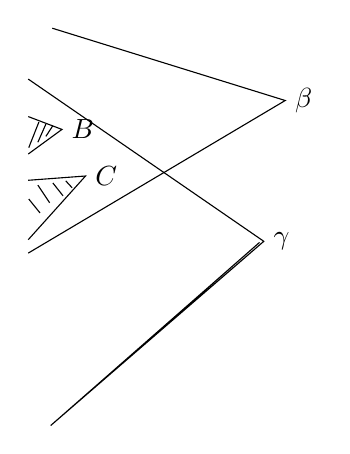
\begin{tikzpicture}[x=.68cm,y=.68cm]
\draw (.45,5.8)--(4.8,4.45)--(0,1.6);
\draw (0,4.85)--(4.4,1.82)--(.42,-1.62)--(4.32,1.8);
\node[right] at (4.8,4.45) {$\beta$}; \node[right] at (4.4,1.82) {$\gamma$};
\draw (0,4.15)--(.63,3.91)--(0,3.45);
\draw (.20,4.05)--(.01,3.57) (.33,4.01)--(.18,3.67) (.46,3.98)--(.33,3.78);
\node[right] at (.63,3.91) {$B$};
\draw (0,2.96)--(1.07,3.04)--(0,1.85);
\draw (.01,2.61)--(.22,2.35) (.18,2.87)--(.40,2.54) (.46,2.91)--(.65,2.67) (.7,2.95)--(.82,2.82);
\node[right] at (1.07,3.04) {$C$};
\end{tikzpicture}}}

% @ middle centre, two tiers of strokes | diagram
\diagram{\handwritten{\begin{tikzcd}[ampersand replacement=\&,row sep=tiny,column sep=tiny]
 \& {}\\
 {}\arrow[ur]\arrow[r] \& {}\\
 {}\arrow[ur,no head]\arrow[r,no head] \& \circ\arrow[d,no head]\\
 \deleted{\unsure{a}}\arrow[r] \& b\arrow[dr,no head]\\
 \phantom{x}\arrow[rr] \& \& x
\end{tikzcd}}}

% @ middle right, line above the vertical pair | display
\[
 \handwritten{\pi_0(\unsure{\mathcal E|\varepsilon|E}_{/x})\simeq}
\]

% @ middle right, vertical pair | diagram
\diagram{\handwritten{\begin{tikzcd}[ampersand replacement=\&]
 \operatorname{Hom}(a,x)\times\mathcal E\arrow[d,shift right]\arrow[d,shift left,no head]\\
 \operatorname{Hom}(a,a)\times\mathcal E
\end{tikzcd}}}

% @ lower third, heading and lines 1–7 | text
\handwritten{\uline{Lemme} Soit $X$ \deleted{dans} Cat \deleted{\unsure{catégorie ayant}} avec quatre objets $B,\ C,\ \beta,\ \gamma$ telle que $\operatorname{Hom}(B,\beta)$, $\operatorname{Hom}(B,\gamma)$, $\operatorname{Hom}(C,\beta)$, $\operatorname{Hom}(C,\gamma)$ \unsure{sont|soient} $\ne\varnothing$, que $B\times C\unsure{=|\ne}\varnothing_{X^\wedge}$ i.e $\nexists x$ \inserted{$\in\operatorname{Ob}X$} avec $\operatorname{Hom}(x,B)\ne\varnothing$ et $\operatorname{Hom}(x,\unsure{e|C})\ne\varnothing$, et $\beta\amalg\gamma=\varnothing_{X^\vee}$ i.e. n'existe pas de $y\in\operatorname{ob}X^\circ$ avec $\operatorname{Hom}(\beta,y)\ne\varnothing$, $\operatorname{Hom}(\gamma,y)\ne\varnothing$. (hyp auto duales). Alors $X$ n'est pas $1$-connexe.}
% slanted
\margin{\handwritten{faux, il faut au moins \deleted{\unsure{supp}} supposer \unsure{en un|en un obj} $x$ tel que $\operatorname{Hom}(x,\beta\times\gamma)\ne\varnothing$, \unsure{on a} $\operatorname{Hom}(x,B)\ne\varnothing$ ou $\operatorname{Hom}(x,C)\ne\varnothing$}}

% @ bottom left, four objects and intervening point | diagram
\diagram{\handwritten{\begin{tikzcd}[ampersand replacement=\&,column sep=small,row sep=tiny]
 B\arrow[dr] \& \& \beta\\
 \& \circ\arrow[ur]\arrow[dr] \& \\
 C\arrow[ur] \& \& \gamma
\end{tikzcd}}}
% archive sheet number: 61
\scanpage{63}
\mspage{\textcircled{3}}
% Reverse-side printing shows through backwards.
% @ upper left, fork with hatched regions | diagram
\diagram{\begin{tikzcd}[ampersand replacement=\&,row sep=tiny]
 \& b\,\tikz[baseline=-.5ex,scale=.33]{\draw (0,0)--(2,0) (0,.05)--(1.4,.55); \draw (.6,.07)--(.8,.28) (1,.08)--(1.33,.47) (1.5,.07)--(1.74,.35);}\\
 a\arrow[ur,no head]\arrow[r,"u"]\arrow[dr] \& x\\
 \& c\,\tikz[baseline=-.3ex,scale=.33]{\draw (0,0)--(2,.12) (0,-.1)--(2.1,-.4); \draw (.62,-.15)--(.85,.04) (1,-.2)--(1.27,.08) (1.43,-.26)--(1.72,.06) (1.85,-.31)--(2.1,.02);}
\end{tikzcd}}

% @ top right, first line | display
\[
 \operatorname{Hom}(a,x)=\varnothing
\]

% @ upper third, line 2 | display
\[
 (u,\beta)\in\operatorname{Hom}(a,x)\times\unsure{\mathcal E|\varepsilon|E}
 \qquad\text{mais alors }\pi_0(\unsure{b|S}_{/x})=\varnothing
\]

% @ upper middle, link above first box | diagram
\diagram{\begin{tikzcd}[ampersand replacement=\&,row sep=small]
 {}\arrow[d,leftrightarrow,"\text{i.e.}"]\\ {}
\end{tikzcd}}

% @ middle, first box | display
\[
 \boxed{e\backslash X=\deleted{\unsure{X}}Z
   ={}_{\beta\backslash\backslash}Z
   \underset{\substack{T\\\Vert\\{}_{B\backslash\backslash}Z\amalg{}_{C\backslash\backslash}Z}}{\amalg}
   {}_{\gamma\backslash\backslash}Z}
\]

% @ middle, second box | display
\[
 \boxed{\begin{aligned}
 \pi_0(S_{/x})&\simeq\deleted{\unsure{\varnothing}} I(x)\amalg(J(x)\times\mathcal E)
          &\mathcal E&=\{\beta,\gamma\}\\
 I(x)&=\operatorname{Im}\bigl(\operatorname{Hom}(b,x)\amalg\operatorname{Hom}(c,x)\to\operatorname{Hom}(a,x)\bigr)\\
 J(x)&=\operatorname{Hom}(a,x)\backslash J(x) &&\unsure{\mathcal E\mathrm c|\mathcal E}
 \end{aligned}}
\]

% @ below boxes, line 1 | display
\[
 \pi_0(b_{/x})=\varnothing\quad\text{si }\operatorname{Hom}(a,x)=\varnothing
\]

% @ lower middle, next three lines | display
\[
 \begin{aligned}
 &\text{Soit}\qquad\unsure{\xi|\zeta}=\operatorname{cl}(u,\alpha)\in\operatorname{Ob}Z,
       &&u:\operatorname{Hom}(a,x)\\
 &&&\alpha\in\mathcal E=\{\beta,\gamma\}\\
 &\hspace{3em}\text{Alors }\exists\ \alpha\longrightarrow\xi\\
 &\text{i.e.}\qquad\xi\in{}_{\alpha\backslash\backslash}Z
 \end{aligned}
\]

% @ bottom right, diamond | diagram
\diagram{\begin{tikzcd}[ampersand replacement=\&,row sep=small,column sep=small]
 \& Z:\,{}_{e\backslash}X\overset{h}{\sim}\unsure{S1|S^1}\arrow[dl]\arrow[dr] \&\\
 \substack{\deleted{\unsure{\varnothing}}\\\text{asph.}}\ e\arrow[dr] \& \& X\ \text{asph.}\arrow[dl]\\
 \& X'\sim S^2 \&
\end{tikzcd}}

% @ bottom left, last line | display
\[
 X'\sim\Sigma^1 Z
\]
% archive sheet number: 62
\scanpage{64}
% letterhead
% @ upper left, printed emblem | drawing
\figure{
\begin{tikzpicture}[x=.19cm,y=.19cm,line width=1.6pt,line cap=butt,line join=miter]
\draw (0,0)--(0,6) (6,0)--(6,6);
\draw (1,6)--(1,3.5)--(5,3.5)--(5,6) (2,6)--(2,4.5)--(4,4.5)--(4,6);
\draw (1,0)--(1,2.5)--(5,2.5)--(5,0) (2,0)--(2,1.5)--(4,1.5)--(4,0);
\end{tikzpicture}}

% @ upper left, sender | letter part
CAISSE\\
DE RETRAITE\\
ET DE\\
PRÉVOYANCE\\
HAUSSMANN\\
Institution AGIRC n\textsuperscript{o} 36 agréée par\\
arrêté du Ministère du Travail du 10-5-48

% @ upper right, title and date | letter part
\textbf{INFORMATION AUX RETRAITES}\\
(Mars 1991)

% @ centre, salutation | letter part
Madame, Monsieur,\\

% @ centre and left column, paragraph 1 | text
\margin{La nouvelle valeur du point}
Nous avons l'honneur de vous informer que le Conseil d'administration de l'AGIRC a porté la valeur annuelle du point à 2,179 F au 1er Janvier 1991 en adoptant une augmentation de 4,11 \% par rapport à la valeur moyenne du point pour l'année 1990.

% @ centre, paragraph 2 | text
Cette nouvelle valeur tient compte d'un recalage sur l'évolution des prix observée au cours des trois dernières années et, en particulier, de l'accélération constatée dès l'été dernier et d'une augmentation moyenne des prix de 1991.

% @ centre, paragraph 3 | text
Cette revalorisation est faite, en principe, pour toute l'année 1991.

% @ lower middle, paragraph 4 | text
L'allocation qui vous sera payée le 2 Avril 1991 au titre du 1er trimestre 1991 tiendra compte de cette nouvelle valeur de point.

% @ lower third, paragraph 5 and left column | text
\margin{La CSG}
Nous vous informons également que la Loi de finances pour 1991 a instauré une contribution sociale généralisée (C.S.G) au profit de la Sécurité sociale.

% @ lower third, paragraph 6 | text
Celle-ci doit être retenue à la source, sur les arrérages versés \textbf{à partir du 1er Février 1991.}

% @ lower third, paragraph 7 | text
En conséquence, toutes les sommes payées par nos services depuis cette date, qu'il s'agisse d'arrérages trimestriels ou de rappels, sont soumises à une retenue supplémentaire.

% @ lower third, paragraph 8 | text
Cette retenue de 1,10 \% est assise sur le montant brut de la retraite versée \textbf{(y compris les majorations pour enfants)}, et \textbf{n'est pas déductible des revenus imposables.}

% @ foot, contact line | letter part
Bureaux et Réception : 64 bis, rue de Monceau 75378 Paris cedex 08 - Tél. : (1) 45.63.79.10\\
Nos collaborateurs pratiquant l'horaire personnalisé, la réception de nos participants est assurée du lundi au vendredi de 9 h 30 à 11 h 55 et de 13 h 25 à 16 h 30 ou sur rendez-vous.
% archive sheet number: 63
\scanpage{65}
% @ top, boxed paragraph | text
\fbox{\parbox{.91\linewidth}{La CSG sera donc réincorporée dans le montant net à déclarer qui figurera sur la déclaration fiscale que nous vous adresserons début 1992 pour vos revenus de 1991.}}

% @ upper third, left label and heading | text
\margin{Les personnes exonérées de la CSG}
Sont exonérés de la CSG :

% @ upper third, first dash | text
- les retraités fiscalement non domiciliés en France

% @ upper third, indented paragraph | text
\textbf{A titre transitoire}, il a été admis que les personnes domiciliées à l'étranger seraient réputées être dans cette situation (sans avoir dans l'immédiat à fournir d'autre preuve).

% @ upper third, second dash | text
- Les retraités :

% @ middle, first dot | text
. dont la cotisation d'impôt sur les revenus de l'année précédente n'est pas mise en recouvrement,

% @ middle, second dot | text
. titulaires d'un avantage vieillesse non contributif attribué sous conditions de ressources.

% @ middle, paragraph after list | text
Ces cas d'exonération sont donc identiques à ceux retenus pour la cotisation \textquotedbl{}\textbf{assurance-maladie}\textquotedbl{} de \textbf{2,40 \% cotisation qui reste toujours applicable}, mais les périodes d'exonération sont différentes.

% @ middle, first Si paragraph | text
Si vous êtes actuellement exonéré(e) de la retenue assurance maladie, vous le serez également pour la CSG.

% @ middle, second Si paragraph | text
Si vous êtes devenu(e) non imposable en 1990 au titre des revenus de 1989 alors que vous l'étiez au titre de l'année précédente et :

% @ lower half, first dash | text
- si vous avez justifié cette situation auprès de la Caisse,(a):

% @ lower half, first dot | text
. vous serez exonéré(e) de la CSG dès le paiement de votre retraite du 1er trimestre 1991,

% @ lower half, second dot | text
. vous ne serez exonéré(e) de la retenue assurance maladie qu'à compter du paiement du 3ème trimestre 1991.

% @ lower third, second dash | text
- si vous n'avez pas justifié encore cette situation auprès de la Caisse, nous vous invitons à le faire pour vous permettre de bénéficier de ces exonérations.

% @ lower third, boxed reminder | text
\fbox{\parbox{.91\linewidth}{Nous vous rappelons que lorsque vous redevenez à nouveau imposable, vous devez en informer la Caisse.}}

% @ foot, note (a) | text
(a) par l'envoi de votre avis de non imposition
% archive sheet number: 64
\scanpage{66}
% @ top, marginal heading and first paragraph | text
\margin{Les dates de paiement en 1991}
Enfin nous profitons de cette lettre d'information pour vous préciser les dates de paiement de vos allocations de retraite en 1991 :

% @ upper third, first date | text
- le 2 Avril 1991 pour le 1er trimestre 1991

% @ upper third, second date | text
- le 1er Juillet 1991 pour le 2ème trimestre 1991

% @ upper third, third date | text
- le 1er Octobre 1991 pour le 3ème trimestre 1991

% @ upper third, fourth date | text
- le 2 Janvier 1992 pour le 4ème trimestre 1991

% @ upper third, final body paragraph | text
Nos services restent bien entendu à votre disposition pour tout renseignement complémentaire.

% @ upper third, closing | letter part
Nous vous prions d'agréer, Madame, Monsieur,\\
l'expression de nos sentiments distingués.\\

% @ middle right, signatory title | letter part
Le Directeur\\

% @ middle right, signature | letter part
\handwritten{\uline{\unsure{Clément} \unsure{Thibéry|Thierry|Thibault}}}\\
% archive sheet number: 65
\scanpage{67}
\mspage{\textcircled{\unsure{4|9}}}
% printed form
% @ top, printed form, left column, lines 1–2 | text
MINISTERE DE L'EDUCATION NATIONALE\\
ACADEMIE D'AIX-MARSEILLE\\
\rule{1cm}{0.3pt}

% @ top, printed form, left column, lines 3–4 | text
Inspection Académique\\
de Vaucluse\\
\rule{1cm}{0.3pt}

% @ top, printed form, left column, lines 5–6 | text
Tél. : 90 82 99 76\\
Référence : Secrétariat n\textsuperscript{o}

% @ top, printed form, right column, line 1 | letter part
AVIGNON, le

% @ top, printed form, right column, lines 2–5 | letter part
L'Inspecteur d'académie,\\
directeur des services départementaux\\
de l'Education Nationale de Vaucluse,\\
à M


% @ beneath form, upper left double diamond | diagram
\diagram{\handwritten{\begin{tikzcd}[ampersand replacement=\&,column sep=small,row sep=small]
 \& (\bar b\amalg\bar c)({}_{a\backslash}X)\arrow[dr] \& \\
 \text{asph.}?\ \deleted{{}_{a\backslash}X}\arrow[ur]\arrow[dr] \& \& {}_{a\backslash}X\ \text{asph. ?}\arrow[dl]\\
 \& {}_{e\backslash}X=Z\arrow[dl]\arrow[dr] \& \\
 \text{asph}\ e\arrow[dr] \& \& e\backslash\deleted{X}\ \text{asph}\arrow[dl]\\
 \& \unsure{\bar X'|X'} \&
\end{tikzcd}}}

% @ upper right, paired lines | diagram
\diagram{\handwritten{\begin{tikzcd}[ampersand replacement=\&]
 \beta\arrow[r] \& \unsure{\xi|\zeta}\\
 a\arrow[r,"u"] \& x \& u,
\end{tikzcd}}}

% @ upper right, fork and circled pair | diagram
\diagram{\handwritten{\begin{tikzcd}[ampersand replacement=\&,row sep=tiny,column sep=small,execute at end picture={\draw (beta.north) .. controls +(1,.15) and +(1,-.3) .. (xx.south) .. controls +(-.55,-.2) and +(-.55,.25) .. cycle;}]
 \& b \& |[alias=beta]|\beta\\
 a\arrow[ur,no head]\arrow[rr,"u"]\arrow[dr,no head] \& \& |[alias=xx]|x\\
 \& c \&
\end{tikzcd}}}

% @ middle right, struck formula | display
\[
 \handwritten{\deleted{{}_{b\amalg_a c\backslash\backslash}\unsure{Z}}}
\]
% @ middle right, above rule | diagram
\diagram{\handwritten{\begin{tikzcd}[ampersand replacement=\&,row sep=tiny]
 \beta\arrow[dr] \&\\
 \&\xi\\
 \gamma\arrow[ur] \&
\end{tikzcd}}}

% @ middle left, above oblique divider | display
\[
 \handwritten{{}_{\beta\backslash\backslash}Z\sim{}_{a\backslash}X}
\]

% @ middle right, below rule | diagram
\diagram{\handwritten{\begin{tikzcd}[ampersand replacement=\&,row sep=tiny,column sep=small]
 \beta\arrow[r]\arrow[dd,no head] \& B\arrow[r] \& \deleted{\unsure{\xi}}x\arrow[dd]\\
 \& b\arrow[dr] \&\\
 a\arrow[ur,very thick]\arrow[rr,"u"]\arrow[dr] \& \& x\\
 \& c\arrow[ur,no head] \&
\end{tikzcd}}}

% @ lower half, stack of three diamonds | diagram
\diagram{\handwritten{\begin{tikzcd}[ampersand replacement=\&,row sep=small,column sep=small]
 \& {}_{(b_0\unsure{\times|,|\amalg}c_0)\backslash\backslash}X_0\arrow[dl]\arrow[dr] \&\\
 {}_{b_0\backslash\backslash}X_0\arrow[dr] \& \substack{\unsure{\mathbb W|W}\\\text{cocart.}} \& {}_{c_0\backslash\backslash}X_0\arrow[dl]\\
 \& T\deleted{={}_{\unsure{(b_0,c_0)}\backslash\backslash}X_0}\arrow[dl]\arrow[dr] \&\\
 X_0={}_{a\backslash}X\arrow[dr,leftrightarrow] \& \substack{\mathbb W\\\text{cocart}} \& {}_{a\backslash}X=X_0\arrow[dl]\\
 \& {}_{e\backslash}X\overset{\unsure{\mathrm{def}|\text{déf}}}{=}\widetilde X\arrow[dl]\arrow[dr,"\text{coét.}"] \&\\
 e\arrow[dr] \& \substack{\mathbb W\text{-}\\\text{cocart}\\!} \& X\arrow[dl]\\
 \& X' \&
\end{tikzcd}}}

% @ lower right, cancellation above T | display
\[
 \handwritten{\deleted{{}_{b\amalg_a c\backslash}\unsure{X}}\,X}
\]

% @ lower right, level with T and X0 | display
\[
 \begin{aligned}
 \handwritten{T={}_{b_0\backslash\backslash}X_0\cup{}_{c_0\backslash\backslash}X_0}\\
 \handwritten{X_0\simeq{}_{\beta\backslash\backslash}\widetilde X\simeq{}_{\gamma\backslash\backslash}\widetilde X}
 \end{aligned}
\]

% @ bottom right, equations either side of vertical divider | display
\[
 \left.\begin{aligned}
 \handwritten{\widetilde X\sim\Sigma^1 T}\\
 \handwritten{X'\sim\Sigma^1\widetilde X}
 \end{aligned}\right|\qquad\handwritten{X'\sim\Sigma^2 T}
\]
% archive sheet number: 66
\scanpage{68}
% @ full sheet, long cancellation strokes | drawing
\figure{\begin{tikzpicture}[x=.41cm,y=.41cm]
\draw[thin] (1.1,7.8) .. controls (1.0,7.1) and (2.0,3.6) .. (3.1,.3);
\draw[thin] (4.6,8.7) .. controls (4.5,6.7) and (5.9,2.2) .. (6.0,.5);
\draw[thin] (7.0,9.0) .. controls (6.45,7.4) and (7.2,3.35) .. (7.8,1.55);
\end{tikzpicture}}
% @ top left | display
\[
 \Sigma^1 X
\]
% @ top centre, pair and arrow | diagram
\diagram{\begin{tikzcd}[ampersand replacement=\&,row sep=tiny,column sep=tiny]
 \& (X,e)\arrow[dl]\\ e \&
\end{tikzcd}}

% @ upper left, double cone with hatched section | drawing
\figure{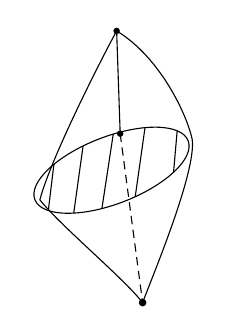
\begin{tikzpicture}[scale=.75,line join=round]
\coordinate (t) at (.04,2.48); \coordinate (b) at (.48,-2.12);
\draw (t) .. controls (.77,2.04) and (1.23,1.07) .. (1.32,.64)
 .. controls (1.39,.09) and (.64,-1.69) .. (b)
 .. controls (.14,-1.69) and (-.91,-.82) .. (-1.26,-.38)
 .. controls (-1.07,.34) and (-.20,2.04) .. (t);
\begin{scope}[rotate=21]
\draw (0,.13) ellipse (1.39 and .57);
\begin{scope}
\clip (0,.13) ellipse (1.39 and .57);
\draw (-1.39,-.40)--(-.75,.81) (-.98,-.54)--(-.19,.89) (-.46,-.55)--(.36,.89) (.16,-.53)--(.96,.91) (.87,-.48)--(1.46,.73);
\end{scope}\end{scope}
\draw (t)--(.10,.74);\draw[densely dashed] (.10,.74)--(b);
\fill (t) circle (.055) (.10,.74) circle (.055) (b) circle (.065);
\end{tikzpicture}}

% @ upper centre, open diamond | diagram
\diagram{\begin{tikzcd}[ampersand replacement=\&,row sep=tiny,column sep=tiny]
 \& {}\arrow[dl,no head]\arrow[dr,no head] \&\\
 \bullet \& \& \cdot\\
 \& {}\arrow[ul,no head]\arrow[ur,no head] \&
\end{tikzcd}}

% @ centre left | diagram
\diagram{\begin{tikzcd}[ampersand replacement=\&,row sep=tiny]
 \&\deleted{X\times Y}\arrow[dl]\\ {} \&
\end{tikzcd}}

% @ centre, small pair | display
\[
 \deleted{\unsure{x,y|x,y'}}
\]

% @ centre right, four-vertex diagram | diagram
\diagram{\begin{tikzcd}[ampersand replacement=\&,row sep=small,column sep=small]
 \& X_0\arrow[dl]\arrow[dr,no head] \&\\
 X_1\arrow[dr] \& \& X_2\arrow[dl]\\
 \& X_3 \&
\end{tikzcd}}

% @ lower left | diagram
\diagram{\begin{tikzcd}[ampersand replacement=\&]
 X\arrow[r] \& \deleted{X\times I}
\end{tikzcd}}

% @ lower right | display
\[
 \deleted{x_0\times I}
\]
% archive sheet number: 67
\scanpage{69}
\mspage{\textcircled{5}}
% @ top left, diamond | diagram
\diagram{\begin{tikzcd}[ampersand replacement=\&,row sep=small,column sep=small]
 \& X_{/F}\simeq X_{/e}\arrow[dl]\arrow[dr] \&\\
 X\arrow[dr,leftrightarrow,"\mathrm{ouv}"'] \& \& e\arrow[dl,"\mathrm{ferm}"]\\
 \text{coasph.} \& X' \&
\end{tikzcd}}

% @ top middle | display
\[
 \unsure{\mathbb X|X}
\]

% @ upper middle, below X | deletion
\deleted{\unsure{X|F}}
% @ upper left, cancelled small sketch | drawing
\figure{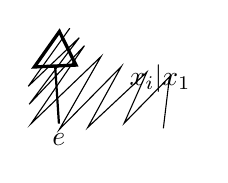
\begin{tikzpicture}[scale=.6]
\draw[very thick] (-.44,1.03)--(.09,1.78)--(.44,1.07)--cycle;
\draw[thick] (0,1.05)--(.08,-.17) node[below] {$\deleted{e}$};
\node at (2.22,.78) {$\deleted{\unsure{x_i|x_1}}$};
\draw (.31,1.85)--(-.57,.62)--(.51,1.65)--(-.55,.24)--(.62,1.48)--(-.51,-.17)
--(.97,1.25)--(.09,-.29)--(1.4,1.04)--(.69,-.25)--(1.94,.92)--(1.46,-.16)--(2.42,.82)--(2.29,-.27);
\end{tikzpicture}}
% @ upper centre and bottom of bracket | text
\unsure{totlt|tot.} 0-connexe,
\[
 \mathbb W_2
\]

% @ middle left, two arrows | diagram
\diagram{\begin{tikzcd}[ampersand replacement=\&]a\arrow[r,shift left]\arrow[r,shift right] \& b\end{tikzcd}}
% @ middle left, two cancelled starts | text
\deleted{Soit $W\subset\mathbb W_2$ \unsure{tel que|plus gén. tel que|plus fine que tt}}

\deleted{Soit $\unsure{W_2|W}$}

% @ middle right, statement | text
$X$ 0-connexe, non ps \unsure{filtrant|cofiltrant|filtrante}
\[
 \begin{aligned}
 &\Rightarrow\quad\exists\, X\longrightarrow X'\text{ cofinal,}\\
 &\text{avec }X'\mathrel{\underset{\mathbb W_\infty}{\sim}}\mathbb S^2,\text{ ou du}\\
 &\text{moins avec}\\
 &\qquad H^2(X')\simeq H^2(\mathbb S^2)
 \end{aligned}
\]
\uline{donc} si $W\subset\mathbb W_2$, plus gén. si \deleted{\unsure{$W$ est|$\mathbb W$ est} \unsure{tel|stable}} $f\in W\Rightarrow$
\[
 f^*\colon H^2(T,k)\xrightarrow{\sim}H^2(\mathbb S,k)
\]
($k$ un groupe ab. donné) donc $X$ n'est pas tot. $W$-asph.

% @ lower sheet, inverted, first boxed note | text
% Opposite orientation from the mathematical notes.
\uline{Evelyne} a téléphoné.\\
\unsure{Monnier|Monsieur} voiture\\
16/1 47 29 50 50

% @ lower sheet, inverted, first two addresses | text
\uline{82000}\\
\unsure{Coty|Côté|Coth}\\
\unsure{pvat|privat}\\
60 rue H. Barbusse \quad 16/1 47 21 \unsure{16|46} 21\\
5 Val des \unsure{Bodurs|Bodeurs|Bodeux} \quad 16/1 47 21 07 71

% @ lower sheet, inverted, bracketed address | text
403 Av. de la République\\
\deleted{\unsure{Maison départementale|Maison département.}}\\
Hospice de Nanterre \quad \uline{16/1} \uline{47 69 65 65}

% @ lower sheet, inverted, time and number tables | text
\uline{St Lazare}\quad $14^{\rm h}04-14^{\rm h}\unsure{16|15}$\\
$14^{\rm h}\unsure{19|10}$ --\\
% @ lower sheet, inverted, ruled box | display
\[
\begin{array}{|l|l|l|l}
\hline
16/1&82\,50\,50&9^{\rm h}01-12^{\rm h}54&\big)\\
\hline
\text{Rés}&90\,82\,56\,29&9^{\rm h}40-13^{\rm h}44&\big)\\
\hline
\multicolumn{2}{|l|}{1\,P\,K\,4\,Y.}&\text{Lyon}\\
\cline{1-2}
\multicolumn{2}{|l|}{\text{Alexandre}}&\\
\cline{1-2}
\end{array}
\]
% archive sheet number: 68
\scanpage{70}
% Read with the printed heading upright; archive image is rotated through 180 degrees.
% printed form
% @ top, printed form, left column, lines 1–2 | text
MINISTERE DE L'EDUCATION NATIONALE\\
ACADEMIE D'AIX-MARSEILLE\\
\rule{1cm}{0.3pt}

% @ top, printed form, left column, lines 3–4 | text
Inspection Académique\\
de Vaucluse\\
\rule{1cm}{0.3pt}

% @ top, printed form, left column, lines 5–6 | text
Tél. : 90 82 99 76\\
Référence : Secrétariat n\textsuperscript{o}

% @ top, printed form, right column, line 1 | letter part
AVIGNON, le

% @ top, printed form, right column, lines 2–5 | letter part
L'Inspecteur d'académie,\\
directeur des services départementaux\\
de l'Education Nationale de Vaucluse,\\
à M


% @ below form, square and two oblique arrows | diagram
\diagram{\handwritten{\begin{tikzcd}[ampersand replacement=\&,column sep=large,row sep=small]
 X\arrow[rr,"{u\in W}"]\arrow[d,"{i\in W_S^{\unsure{u|n|\prime\prime}}}"'] \& \&Y\arrow[d,"{j\in W_S^u}"]\\
 \overline X\arrow[rr,"{\overline u\in W}"]\arrow[dr,"{p\in G}"'] \&\&\overline Y\arrow[dl,"{q\in G}"]\\
 \& S \&
\end{tikzcd}}}

% @ below form, right-hand triangle | diagram
\diagram{\handwritten{\begin{tikzcd}[ampersand replacement=\&,column sep=large,row sep=small]
 X\arrow[dr,"{\deleted{i\in} W_S^u}"]\arrow[dd,"{\unsure{\operatorname{Fibf}_u|\operatorname{Fib}f_u}}"'] \&\\
 \&\unsure{L(X)|\mathscr L(X)|\mathcal G(X)}\arrow[dl,"{\unsure{\mathrm{Fib}|\mathrm{Fibr}|F_W}}"]\\
 S \&
\end{tikzcd}}}

% @ below triangle | display
\[
 \handwritten{\overline u\in W_S^u}
\]
% @ midpage right, underlined reference | text
\handwritten{\uline{$\overline{\mathrm{VI}}$}\qquad 171 -- 205}

% @ middle left, fork | diagram
\diagram{\handwritten{\begin{tikzcd}[ampersand replacement=\&]
 X\arrow[r]\arrow[dr]\&{}\\ \&S
\end{tikzcd}}}

% @ lower left, before square | deletion
\handwritten{\deleted{\unsure{Avec|aux}}}
% @ lower left, square | diagram
\diagram{\handwritten{\begin{tikzcd}[ampersand replacement=\&]
 X\arrow[d]\& X'\arrow[l]\arrow[d]\\
 S\& S'\arrow[l,"w"']
\end{tikzcd}}}

% @ lower middle and right, coefficients and cohomology | display
\[
 \handwritten{\unsure{\zeta|\mathcal F|\xi}\qquad\zeta'\qquad H^{\unsure{?|D_{\bullet}|p}}(S',\zeta')\longrightarrow H^{?}(S,\zeta)}
\]
% @ below coefficient letters | display
\[
 \handwritten{\deleted{\unsure{H^{?}_S(\zeta')|H^{?}_D(\zeta')|H^{p}(S,\xi)}}}
\]
% @ bottom, product arrow | diagram
\diagram{\handwritten{\begin{tikzcd}[ampersand replacement=\&]
 S\times T\& S'\times T\arrow[l]
\end{tikzcd}}}
% archive sheet number: 69
